\subsection{Artificial Intelligence in Games}

For games, one of the most important aspects is the player's experience.
The game's flow and immersion are key elements to this experience \cite{ijsselsteijn:userexperience}, and this is where \ac{AI} comes into play.
In the last years, in order to improve player's game play experience, the game industry have used \ac{AI} with several different purposes: player experience modelling, procedural content generation, massive-scale game data mining, and \ac{NPC} \ac{AI} \cite{yannakakis:gameairevisited}.

In this section I'm interested in exploring the techniques and tools used for the creation of \ac{NPC}s.
As the name suggests, non playable characters are part of the game but the player cannot control them.
If not the player, then who controls \ac{NPC}s?
The answer is \ac{AI}.
In games, \ac{AI} focus on the creation of characters that behave like humans or animals.

However, game \ac{AI} doesn't always use complex techniques to achieve believable characters, and often, the more complex algorithms produce behaviours that appear stupid \cite{millington:AIgames}.
For example, in Black and White \cite{game:black&white} the player plays the part of a god.
Using a gigantic creature under his control, the player can take over villages, see Fig. \ref{fig:black-and-white}.
\begin{figure}
  \centering
    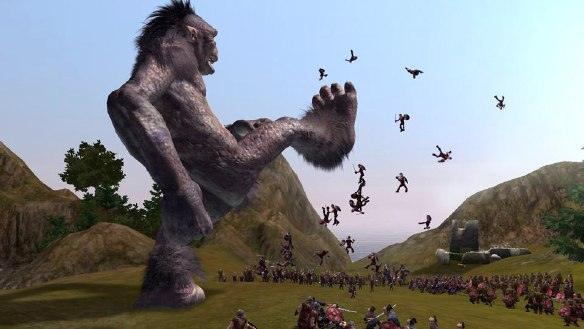
\includegraphics[width=\textwidth]{black-and-white}
  \caption{Black and White, example of using your creature to destroy a village.}
  \label{fig:black-and-white}
\end{figure}
This creature uses reinforcement learning algorithms to learn the behaviours that the player wants him to perform automatically.
But not always the creatures learns want the player wants, learning unwanted behaviours and even failing to learn the most basic ones.

Because of this, and the lack of control on more complex algorithms, game developers sometimes choose to fake it.
"If it looks like a duck, and makes quack, it probably is a duck".
Instead of using complex algorithms, game developers tend to use clever solutions that produce a good behaviour.

In Pacman \cite{game:pacman}, the ghost's behaviour can almost be viewed as each one of them having different personalities.
In Japan, each of them even as a name that characterizes their behaviour almost to the letter: the red ghost, \textit{oikake}, which means "to run down or pursue"; the pink ghost, \textit{machibuse}, meaning "to perform an ambush"; the blue ghost, \textit{kimagure}, meaning "a fickle, moody, or uneven temper"; and the orange ghost, \textit{otoboke}, meaning "pretending ignorance".
By using four different targeting functions (check Fig. \ref{fig:ghosts-targeting})\ref{pacman:dossier}, the game developers have managed to create interesting and challenging opponents that have believable behaviours.

\begin{figure}
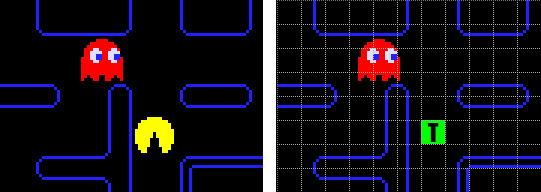
\includegraphics[width=0.5\textwidth]{blinky}
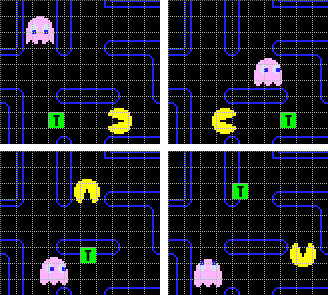
\includegraphics[width=0.5\textwidth]{pinky}
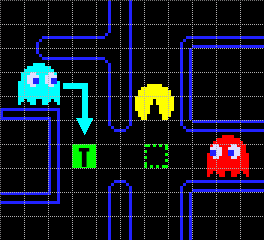
\includegraphics[width=0.5\textwidth]{inky}
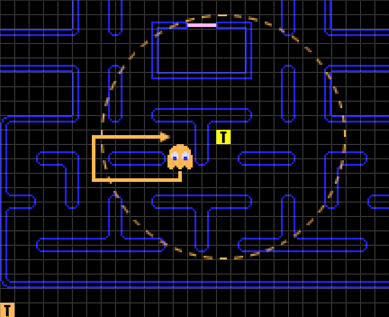
\includegraphics[width=0.5\textwidth]{clyde}
  \caption{Pacman's ghosts targeting functions examples.}
  \label{fig:ghosts-targeting}
\end{figure}

For the remainder of this section I'll follow Millington's work \cite{millington:AIgames} on \ac{AI} for games, exploring three common used techniques: Hacks, Heuristics and Algorithms.
In the end I'll present some common constraints found when building \ac{AI} for games.

\subsubsection{Hacks}
\subsubsection{Heuristics}
\subsubsection{Algorithms}
\subsubsection{Constrains}